% !TEX root = ../mechrelab.tex
\chapter{Characterizing Electronic Components}\label{expt:02-elec-char}
% !TEX root = ../mechrelab.tex

In this lab you will characterize three important electronic components: diode, BJT, and MOSFET. You will learn how to measure their I-V characteristics and understand their behavior in circuits.

This will be followed by you designing, building, and testing simple circuits using these components, and answering questions related to these circuits. 

\section{Circuit 01: Diode I-V Characteristics}
Build the following series RC circuit (Figure~\ref{fig:expt02-01}) on a breadboard and answer the following question:
\begin{figure}[htbp]
    \centering
    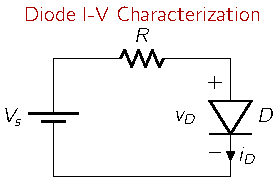
\includegraphics[width=0.5\textwidth]{figures/expt02/expot02-diode-iv.pdf}
    \caption{A diode I-V characteristic circuit.}
    \label{fig:expt02-01}
\end{figure}
\begin{enumerate}
    \item In the above circuit vary the supply voltage $V_s$ from 0 to 5V and measure the diode current $i_D$ and voltage $v_D$ at each supply voltage $V_s$. Choose $R=100\Omega$. Plot the diode I-V characteristics by plotting $i_D$ versus $v_D$, and fit the Schockley diode equation to the data:
    \begin{equation}
        i_D = I_s \left( e^{\frac{v_D}{nV_T}} - 1 \right)
    \end{equation}
    where $I_s$ is the reverse saturation current, $n$ is the ideality factor, and $V_T$ is the thermal voltage (approximately 26mV at room temperature). Estimate the values of $I_s$, $n$, and $V_T$ from your data.
    \item Now reverse the polarity of voltage source $V_s$, and repeat the measurements for negative voltages. Plot the I-V characteristics again, and comment on the behavior of the diode in reverse bias.
\end{enumerate}

\section{Circuit 02: BJT I-V Characteristics}
Build the following $npn$-BJT circuit (Figure~\ref{fig:expt02-01}) on a breadboard and answer the following question:
\begin{figure}[htbp]
    \centering
    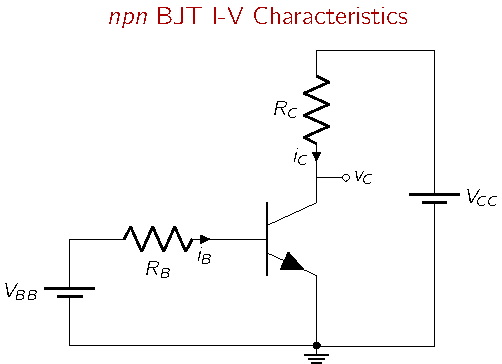
\includegraphics[width=0.65\textwidth]{figures/expt02/expt02-bjt-iv.pdf}
    \caption{A BJT I-V characteristic circuit.}
    \label{fig:expt02-02}
\end{figure}
In the above circuit, fix $R_B = 10k\Omega$, $R_C = 1k\Omega$, and $V_{CC} = 5V$. We will vary $V_{BB}$ from 0 to 5V, and measure $i_B$ and $i_C$ for different values of $V_{BB}$. With this data, answer the following questions:
\begin{enumerate}
    \item Plot the the relationship between $V_{BB}$ and $v_C$. Can you identify the cutoff, active, and saturation regions of the BJT operation from this graph? 
    \item Plot the relationship between $i_B$ and $i_C$. How can you estimate the current gain $\beta$ of the BJT from this graph? How does it compare to the datasheet value?
\end{enumerate}

In the above circuit, if $V_{BB}$ was chosen so that $v_C = 2.5V$. If $V_{BB}$ varied bt $\pm 0.1V$, how much would the collector voltage $v_C$ vary by? Answer this question using the following approaches,
\begin{itemize}
    \item $V_{BB}$ versus $v_C$ data you collected earlier.
    \item The $i_B$ versus $i_C$ data you collected earlier.
\end{itemize}
Experimentally measure the change in $v_C$ for a $\pm 0.1V$ change in $V_{BB}$, and compare it with your predictions from the two approaches above.